\chapter{Experiments and results}
\label{AER}

\section{A Good Curve}
Assuming a very simple model, with no washin or washout rate, a good bacteria growth curve looks like a mountain, with a clear rise, peak, and fall in population levels. 
For a given initial condition, the bacteria start to consume resources and replicate leading to exponential growth. 
The phages start to infect the bacteria and eventually the bacteria start to die, releasing new phages. 
The new phages infect more bacteria, putting pressure on the bacteria growth. 
Eventually, more bacteria are being infected than being created, causing the decline in bacteria population. 
\Cref{fig:created:a_good_curve_linear} shows an example of a good curve. 
\Cref{fig:created:a_good_curve_logarithmic} is the same plot but with a logarithmic y-axis. 

As the bacteria population grow, the resource consumption speeds up until there are trace amount of resources left at $t=8$. 
The uninfected and infected bacteria exhibit exponential growth, peaking at 1617 at $t=3.99$ and 3463 at $t=5.27$ respectively. 
The delay in the uninfected to infected bacteria's peak is due to the infection stages and latent period of the phage infection. 
The bacteria sum do not have as stark of a peak in comparison to the uninfected and infected bacteria, due to the graph measuring all bacteria populations, but the peak of 3805 at $t=4.89$ is still clear. 
The phages saw a significant increase in population count at around $t=4$, coinciding with the peak in uninfected bacteria. 
At this point in time, the infection rate is larger than the bacteria replication rate, so the bacteria are starting to die out even though there are still sufficient resources remaining. 
At around $t=4$ is when the the resource consumption rate inflects. 
The rate at which the resources are being consumed starts to slow down, showing a decreasing sigmoid shape. 
The total bacteria population reached a peak of 3805 at $t=4.89$, a 76.1x increase in population count from the initial 50 starting uninfected bacteria. 
The phage population reached a peak of 2584 phages at $t=15$, a 258.4x increase in population count. 

\begin{figure}[h!]
    \centering
    \begin{subfigure}{1\linewidth}
        \centering
        \captionsetup{width=1\linewidth}
        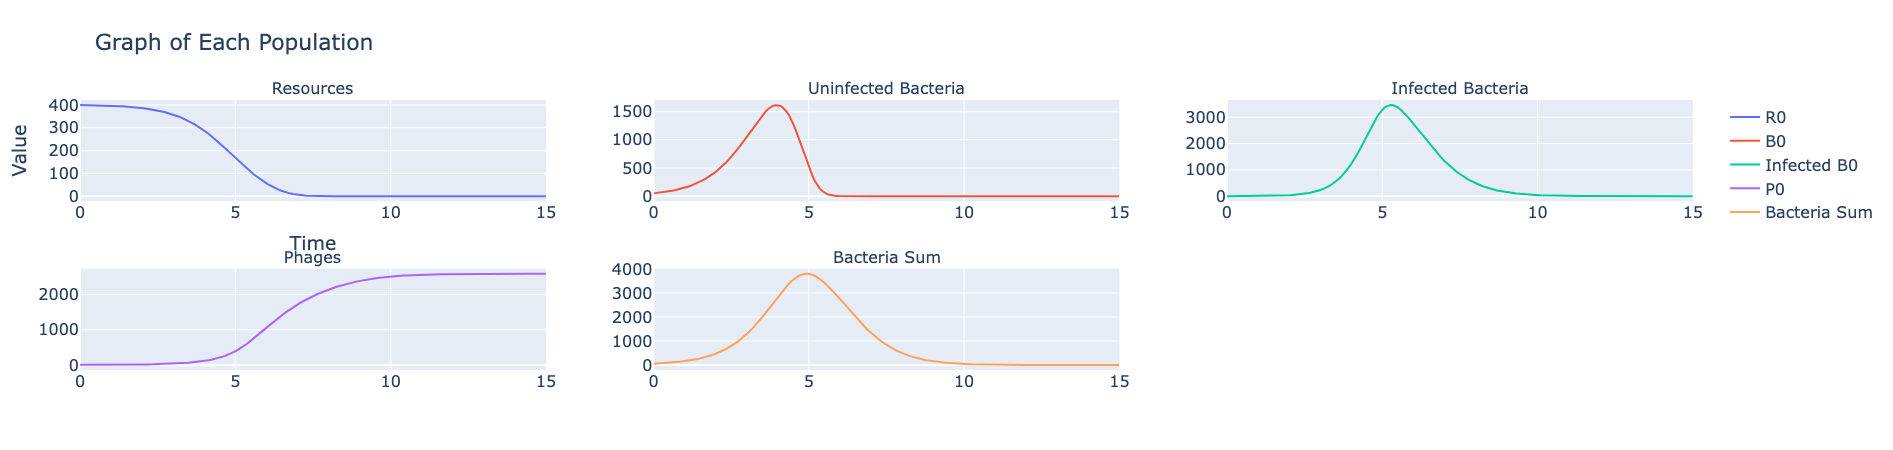
\includegraphics[width=\linewidth]{Plots/Created/a_good_curve_linear.png}
        \caption{
            Linear y-axis for a "good" plot. 
        }
        \label{fig:created:a_good_curve_linear}
    \end{subfigure}
    \hfill
    \begin{subfigure}{1\linewidth}
        \centering
        \captionsetup{width=1\linewidth}
        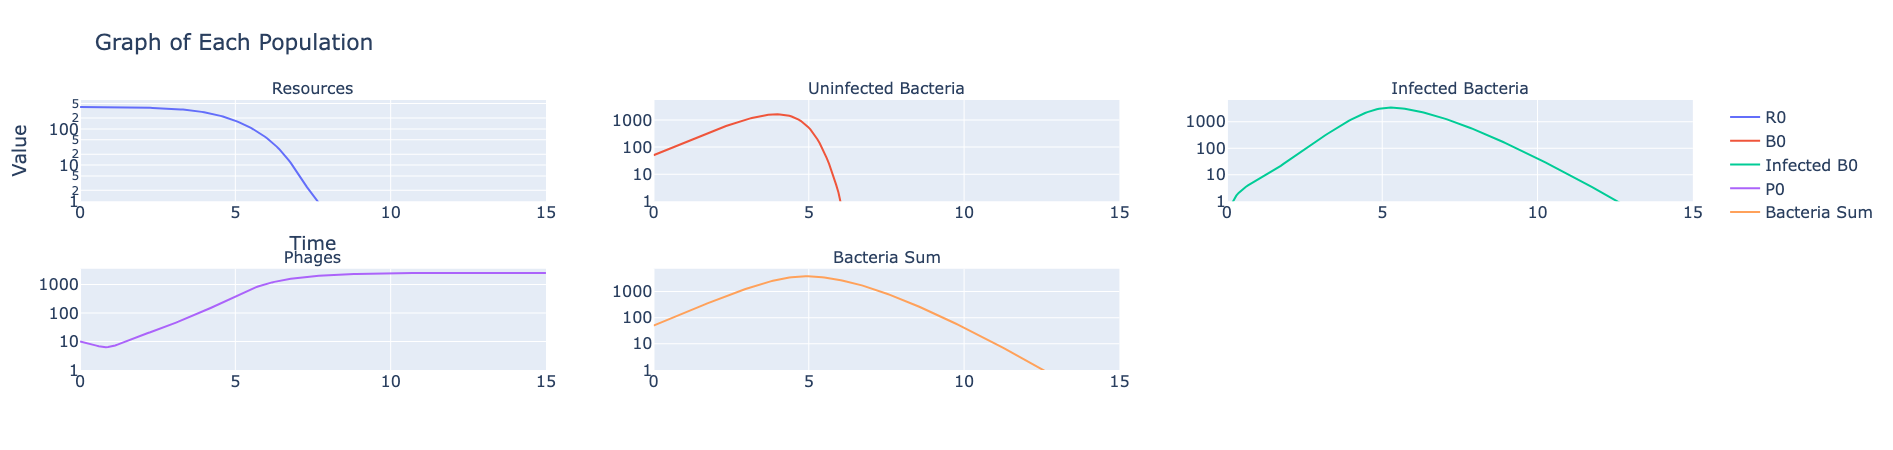
\includegraphics[width=\linewidth]{Plots/Created/a_good_curve_logarithmic.png}
        \caption{
            Logarithmic y-axis for a "good" plot. 
        }
        \label{fig:created:a_good_curve_logarithmic}
    \end{subfigure}
    \caption{
        The log plot allows to see behavior happening at values near 0. 
        The parameters used for this plot can be found in \Cref{tab:appendixE:a_good_curve}. 
    }
    \label{fig:created:a_good_curve}
\end{figure}

\section{SOBOL Sensitivity Analysis Results}
\label{sec:SOBOL_sensitivity_analysis_results}
It is important to understand how a change in parameter value affects the change in output of a model. 
Models will have parameters that are more important and have a larger effect on the model output than other parameters. 

\Cref{fig:created:SOBOL_average} shows the impact that the parameter had on the final value of the population at $t=15$. 
\Cref{fig:created:SOBOL_average} and \Cref{fig:created:SOBOL_variance} show the impact that the parameters had on the average value and variance of the population throughout the simulation respectively. 
The parameters that were tested include all the parameters listed in the extended golden model, except for Uninfected Bacteria and $M$. 
Uninfected Bacteria was left out as it doesn't make sense to already add infected bacteria to the system
$M$, the number of stages that the infection goes through, can not be tested as $M$ hardcodes the number of infection stages that the bacteria has to go through. 
The hardcoding is done before the simulation framework starts. 
As such, it is not possible to change $M$. 

What can immediately be noticed in \Cref{fig:created:SOBOL_default} is how the plots all look very similar. 
There might be some minor differences from bar to bar across plots, but the difference is imperceptible. 
Since the plots all look similar, only an analysis on the final value will be done. 

\subsection{Final Value Analysis}
\subsubsection{Resources}
The $\omega^i$/washin rate had the largest influence on the final, average and variance value. 
Without a washin rate, the resources will most likely have been consumed by the time the simulation ended at $t=15$. 
The final values for Resources, Uninfected, Infected, and Phages would often be something similar to (0, 0, 0, 10000) at $t=15$, where all the resources were consumed and the bacteria died out due to the phages, leaving only the phages remaining. 
The final value of the resources would often be 0, no matter what parameter values were used, with $\omega^i, \omega^o = 0$. 
With the addition of the washin, new resources were constantly being re-added. 
Once the bacteria died out, the resources could accumulate, with the accumulation dependent on the rate of the washin rate, hence why the washin rate has such a large impact on the final, average, and variance of population value for the resources. 
The final value would then be dependent on when the bacteria died out, allowing the resources to accumulate, and the $\omega^i - \omega^0\cdot R$ rate. 
Resources were less dependent on higher order interactions, unlike the uninfected, infected, phages, and total bacteria sum. 

\subsubsection{Uninfected}
The uninfected bacteria population sensitivities depend on many higher order interactions between the parameters as $ST_i >> S1_i$. 
The uninfected are highly dependent on $\beta$/B\_matrix and initial phage population, as the initial phage population will determine how many bacteria become infected, and how quickly the phages can proliferate through the bacteria population. 
Surprisingly, $r$/r\_matrix did not have as big of an influence on the uninfected as $\beta$ did, even though the infection rate is dependent on $r$. 
The larger or smaller $r$ is, the faster or slower the infection rate is. If $r$ is really small, the infection rate would take forever, potentially allowing the bacteria to keep a stable population. 
$r$ is equally as important at explaining the final value as $\tau$/tau\_vector, washin, $e$/e\_matrix, and washout of sensitivity around 0.25. 

\subsubsection{Infected}
Since $ST_i >> S1_i$ for the infected bacteria, where $S1_i \approx 0$ for nearly all of the parameters, the infected bacteria heavily depend on many interactions happening at the same time. 
This makes intuitive sense after looking at \nameref{sec:golden_model}. 
The infected (and uninfected) bacteria directly interact with $R$, $U$, $P$, $v$, $K$, $r$, $\tau$, and $\omega^o$, ($M$ is not included as it was left out of the analysis). 
So due to the high coupling of parameters, the infected (and also the uninfected) have large global sensitivities compared to the local sensitivity. 

However SOBOL had some difficulties assigning a good sensitivity score to each parameter for the $ST$ and $S1$ tests as noticed by the slightly larger error bars in the infected than the uninfected or resources. 
This is most likely due to the infected bacteria going through multiple stages of infection, causing a delay and uncertain behavior in the final value, despite the ODE model being deterministic. 

\subsubsection{Phages}
The most important factor for the final phage value is $r$, followed by $\beta$, $\omega^o$ and $P$. 
The $r$ value allows the phages to infect the uninfected. 
When $r$ is decreased, the final phage population is counterintuitively higher than when $r$ is larger. 
The behavior is counterintuitive because one would expect that a higher infection rate would lead to more infections and thus more phages. 
With a higher $r$ value, more phages are being removed from the phage population and infecting the bacteria. 
It can be seen as a way of "more phages are needed to infect a bacterium", therefore getting less phages out as a result as more phages are needed to infect a single bacteria. 

Washout has a noticeable influence on the phage population, as not the phage population is being reduced at a rate proportional to the washout rate. 
The larger the washout rate, the larger the drawdown of phages. 
When the infected all die out, the phage population wont grow anymore. 
Given the phage population at that point in time, the phage removal rate is proportional to the washout rate. 

\subsubsection{Total Bacteria}
Total bacteria is the sum of both uninfected and infected bacteria, so it makes sense for total bacteria to have similar values to uninfected and infected bacteria. 
Apparently the uninfected bacteria have a stronger influence on the output variance than the infected bacteria. 
The total bacteria sensitivities resemble the sensitivities of the uninfected bacteria more than the infected bacteria. 
It would have been expected for the total bacteria to resemble more of an average between the uninfected and infected. 

\begin{figure}
    \centering
    \begin{subfigure}{0.32\linewidth}
        \centering
        \captionsetup{width=1\linewidth}
        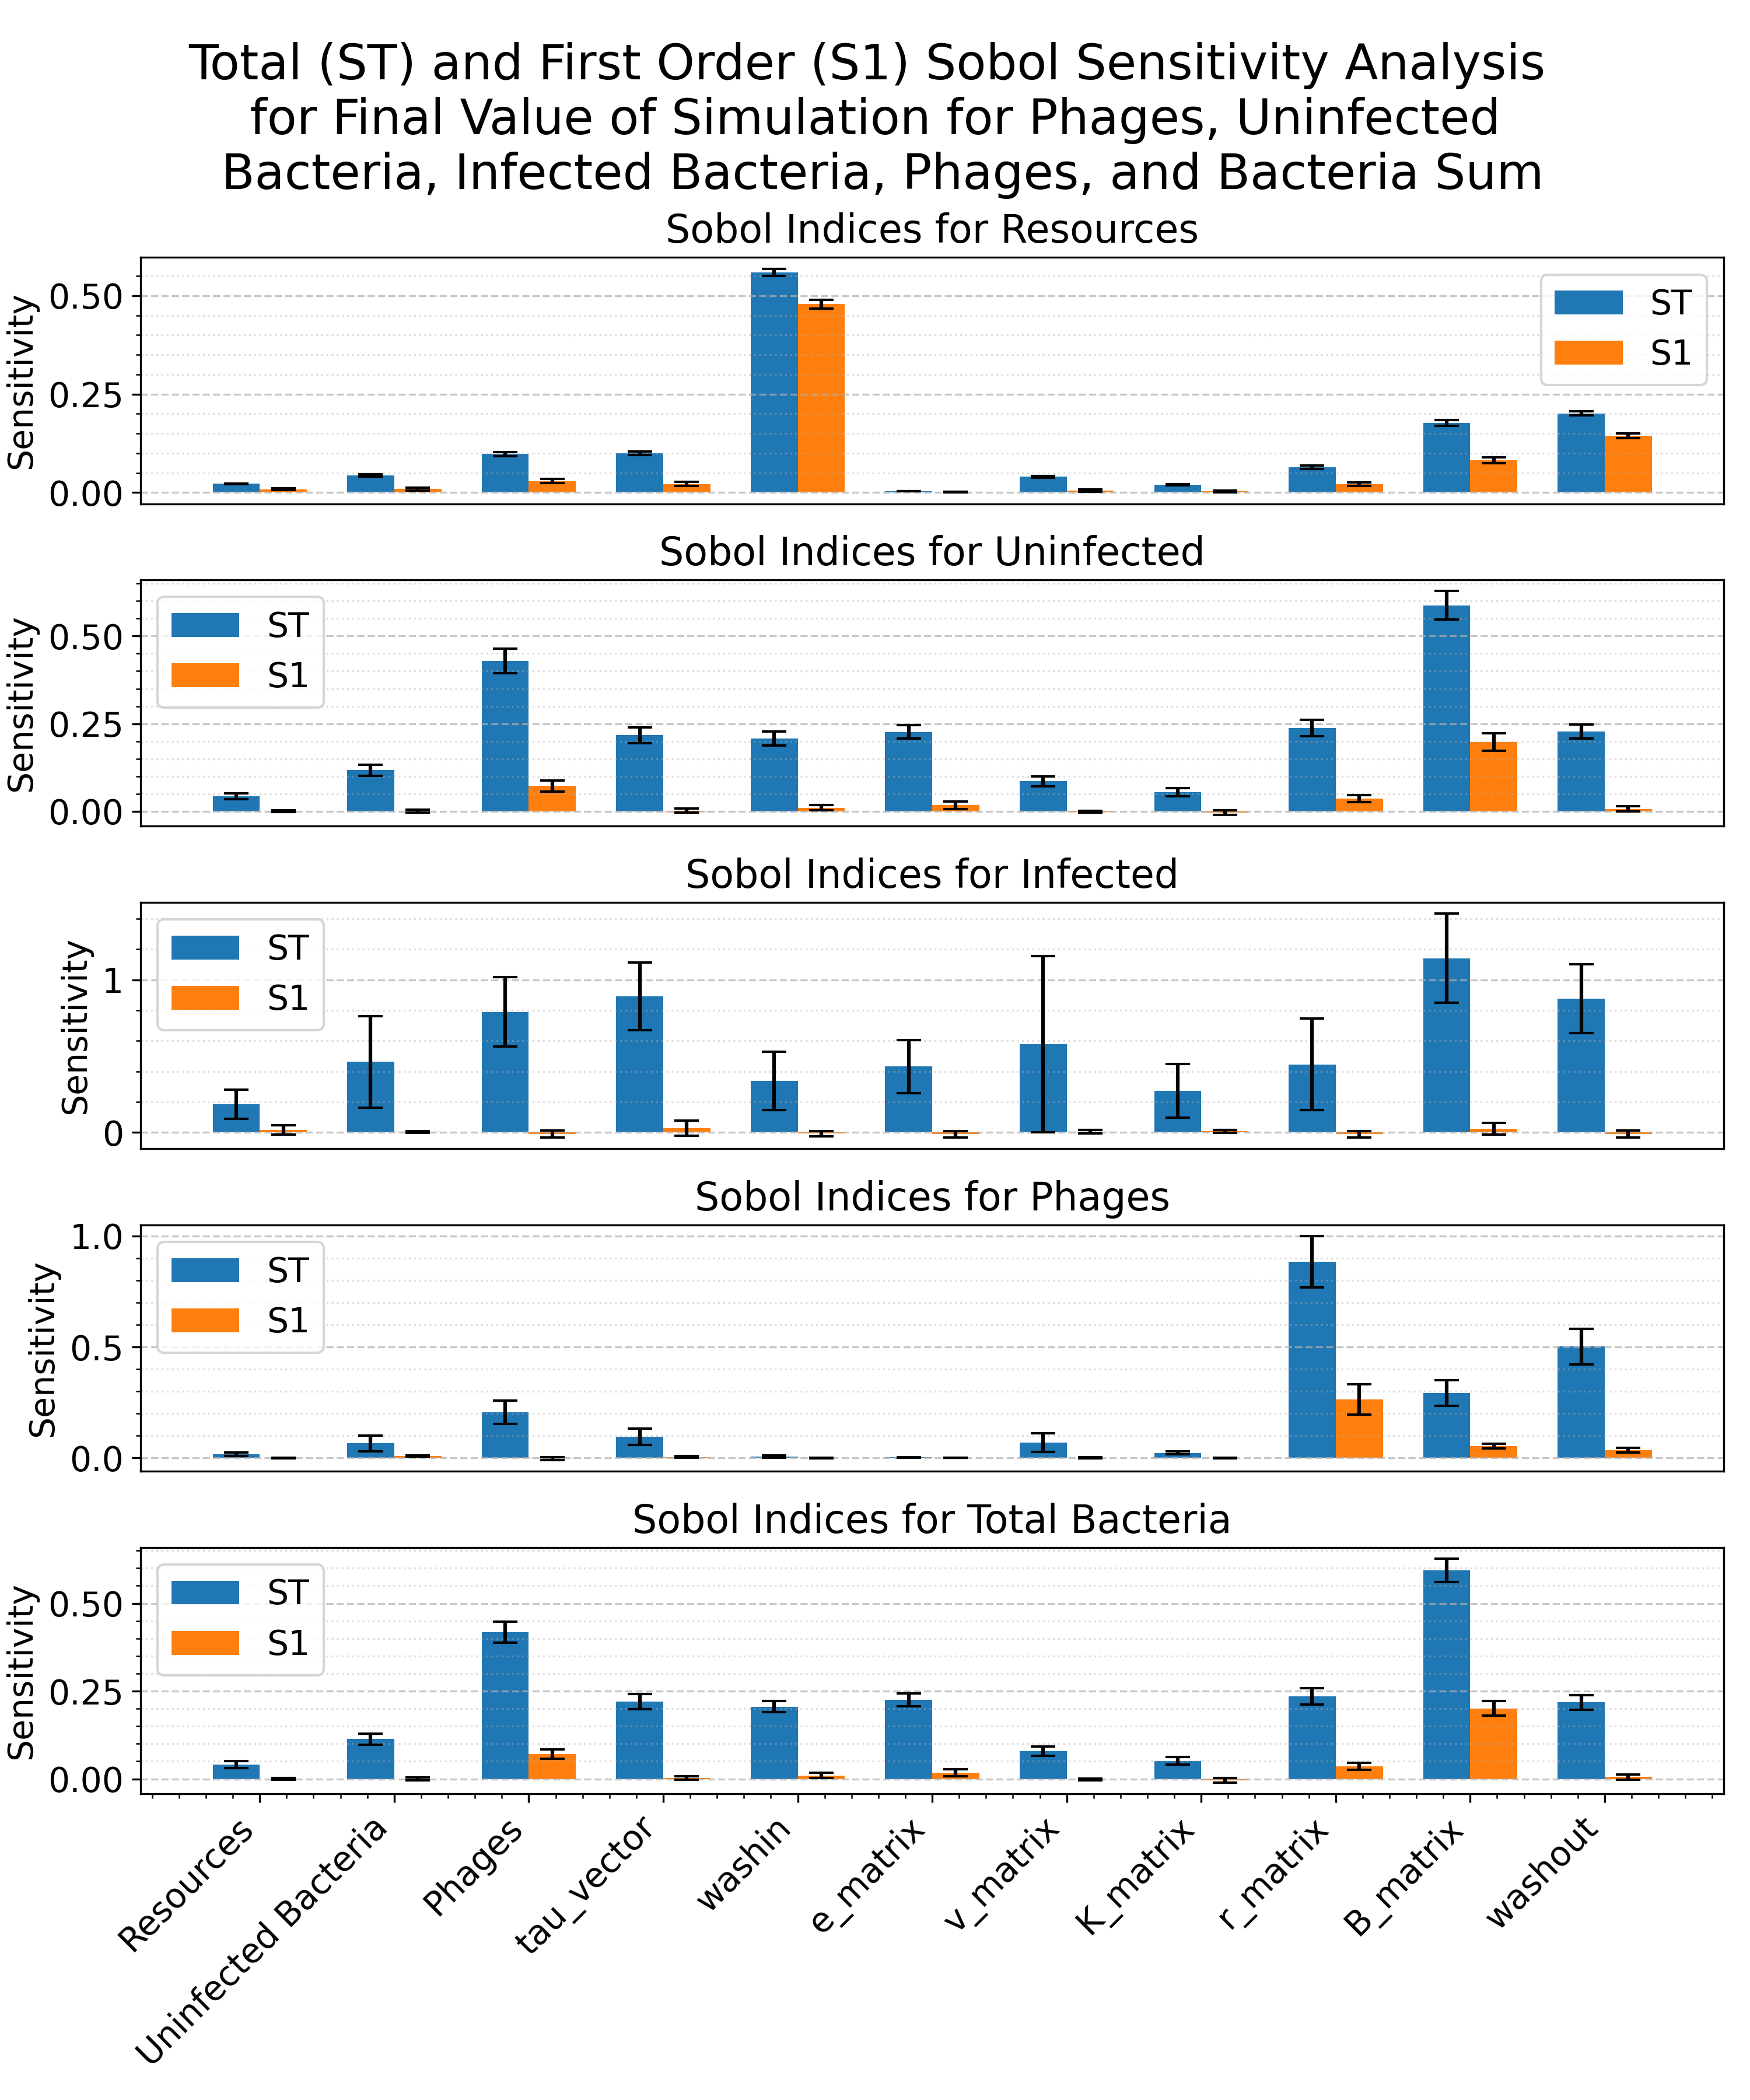
\includegraphics[width=\linewidth]{Plots/Created/SOBOL_analysis_1748084143_Final.png}
        \caption{
            The $ST$ and $S1$ sensitivity for the final Resource, Uninfected, Infected, Phage, and Total Bacteria population. 
        }
        \label{fig:created:SOBOL_final}
    \end{subfigure}
    \hfill
    \begin{subfigure}{0.32\linewidth}
        \centering
        \captionsetup{width=1\linewidth}
        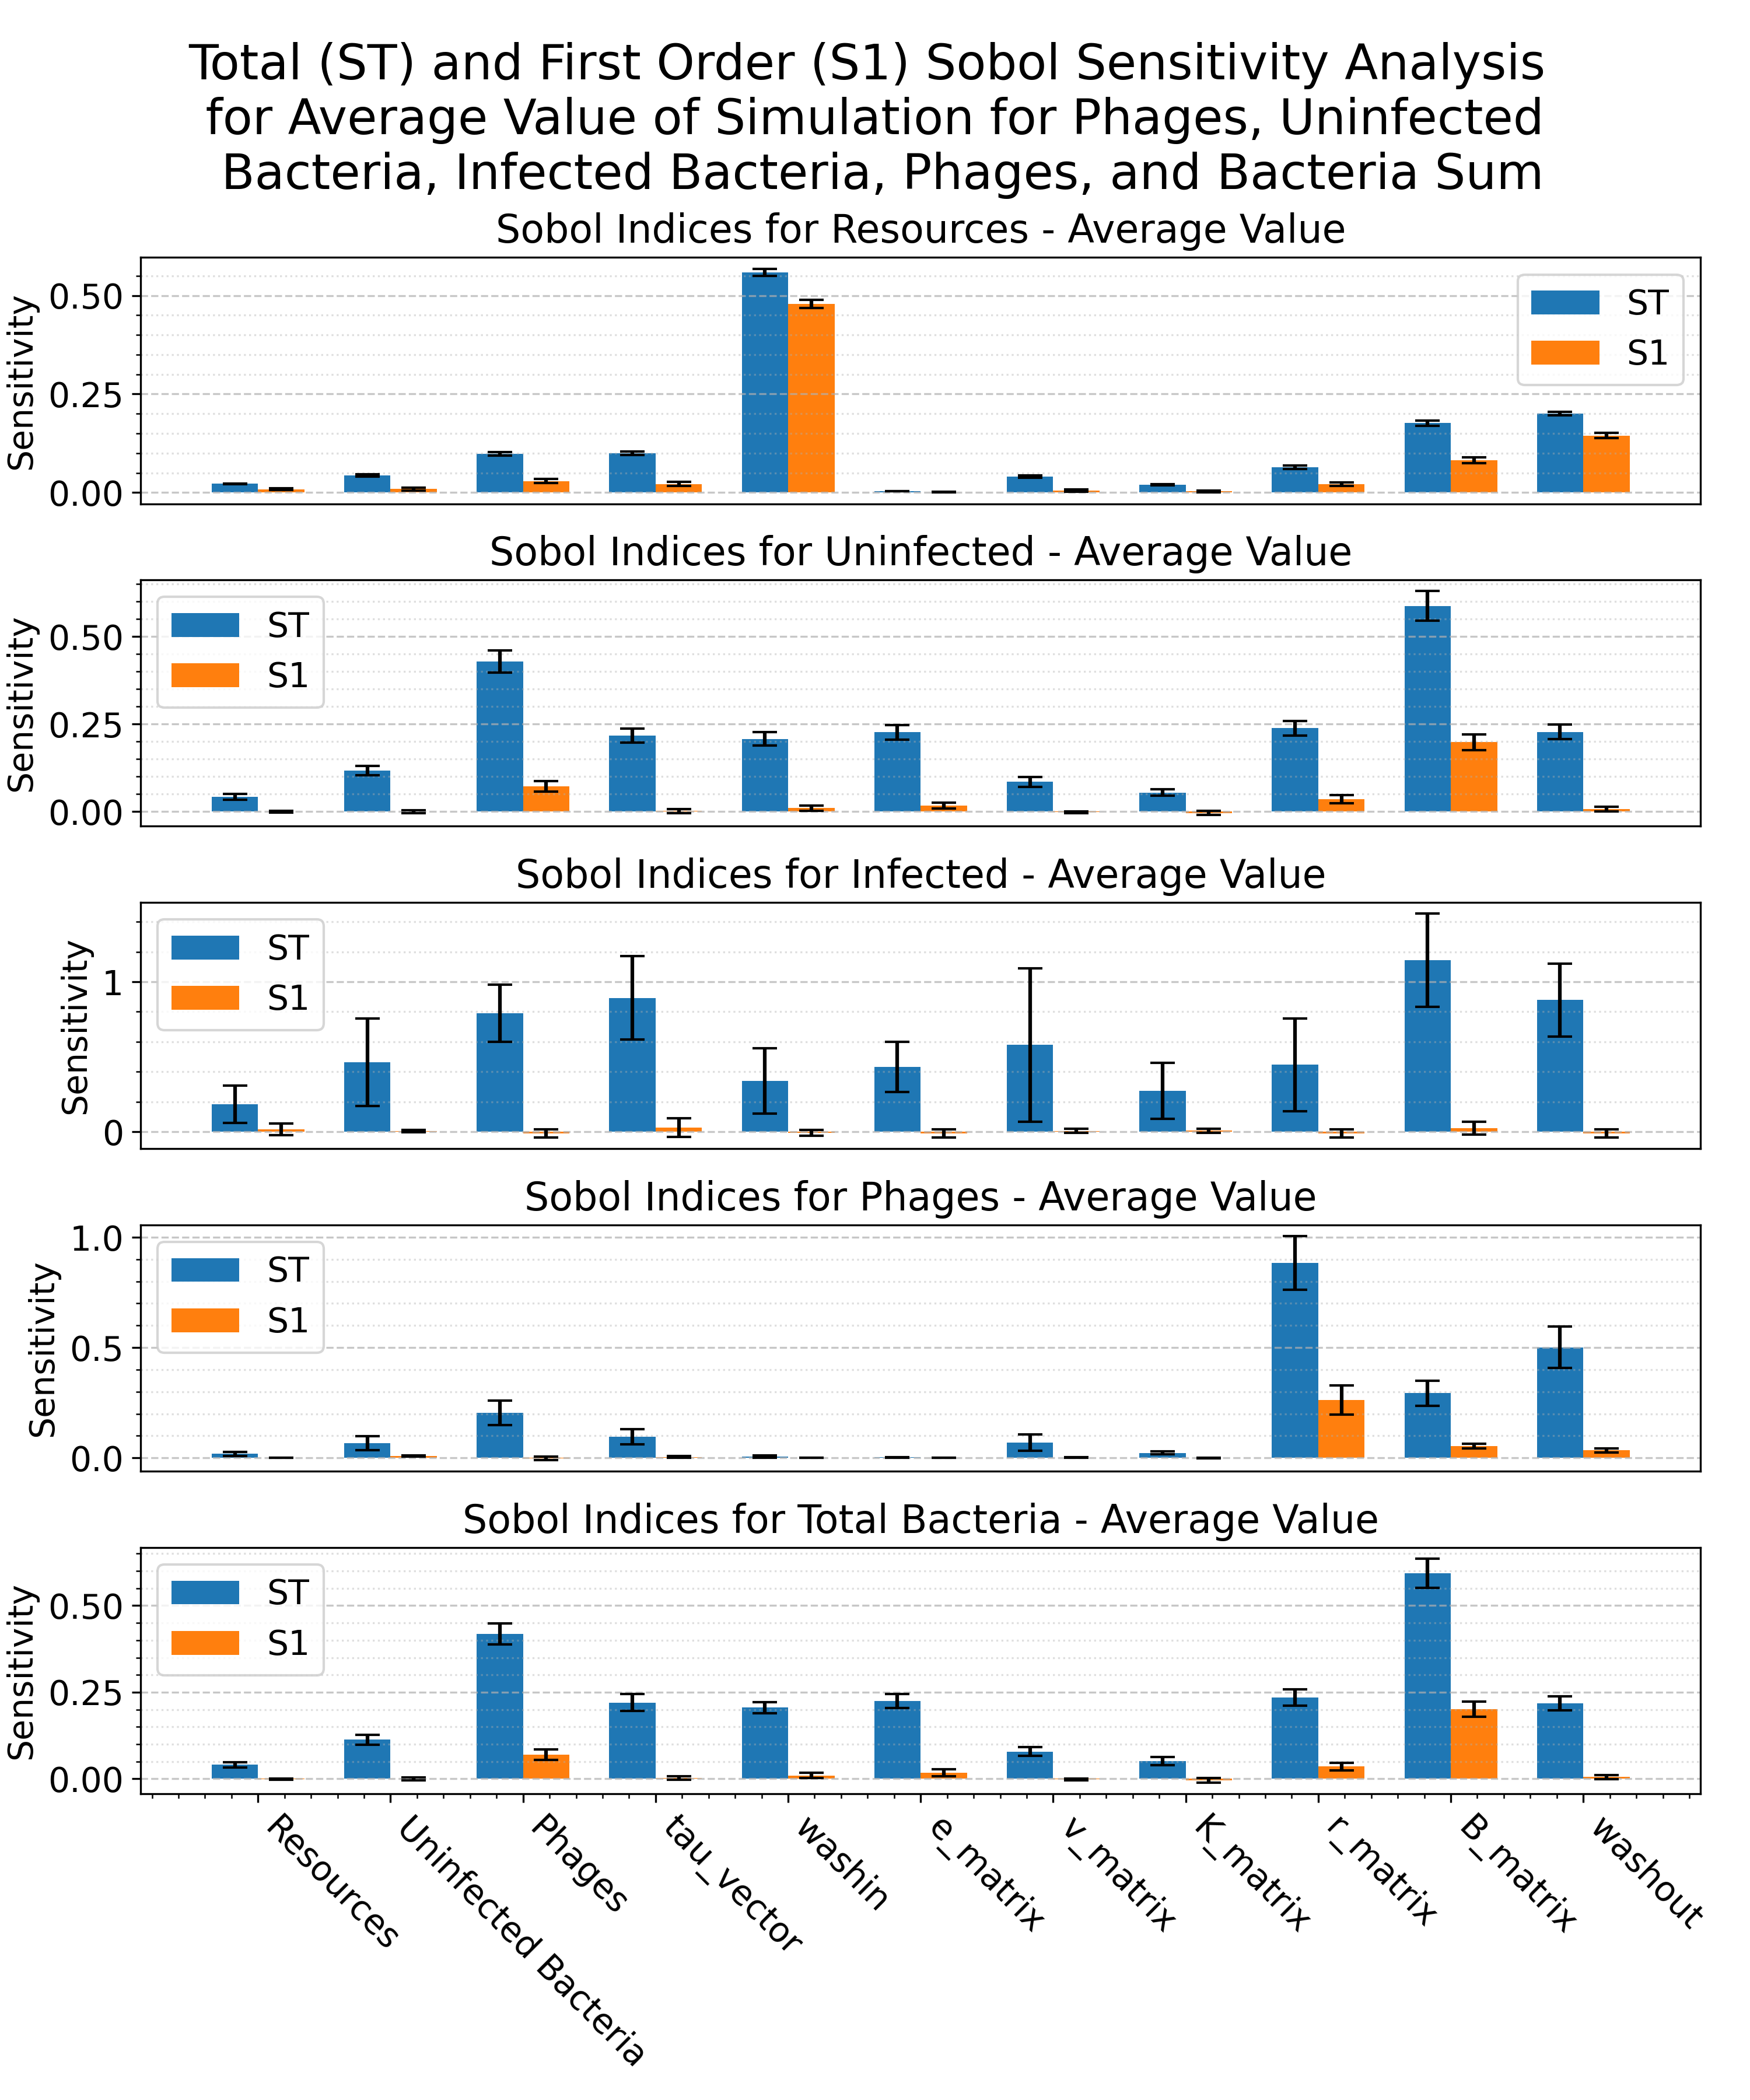
\includegraphics[width=\linewidth]{Plots/Created/SOBOL_analysis_1748084143_Average.png}
        \caption{
            The $ST$ and $S1$ order sensitivity for the average Resource, Uninfected, Infected, Phage, and Total Bacteria population. 
        }
        \label{fig:created:SOBOL_average}
    \end{subfigure}
    \hfill
    \begin{subfigure}{0.32\linewidth}
        \centering
        \captionsetup{width=1\linewidth}
        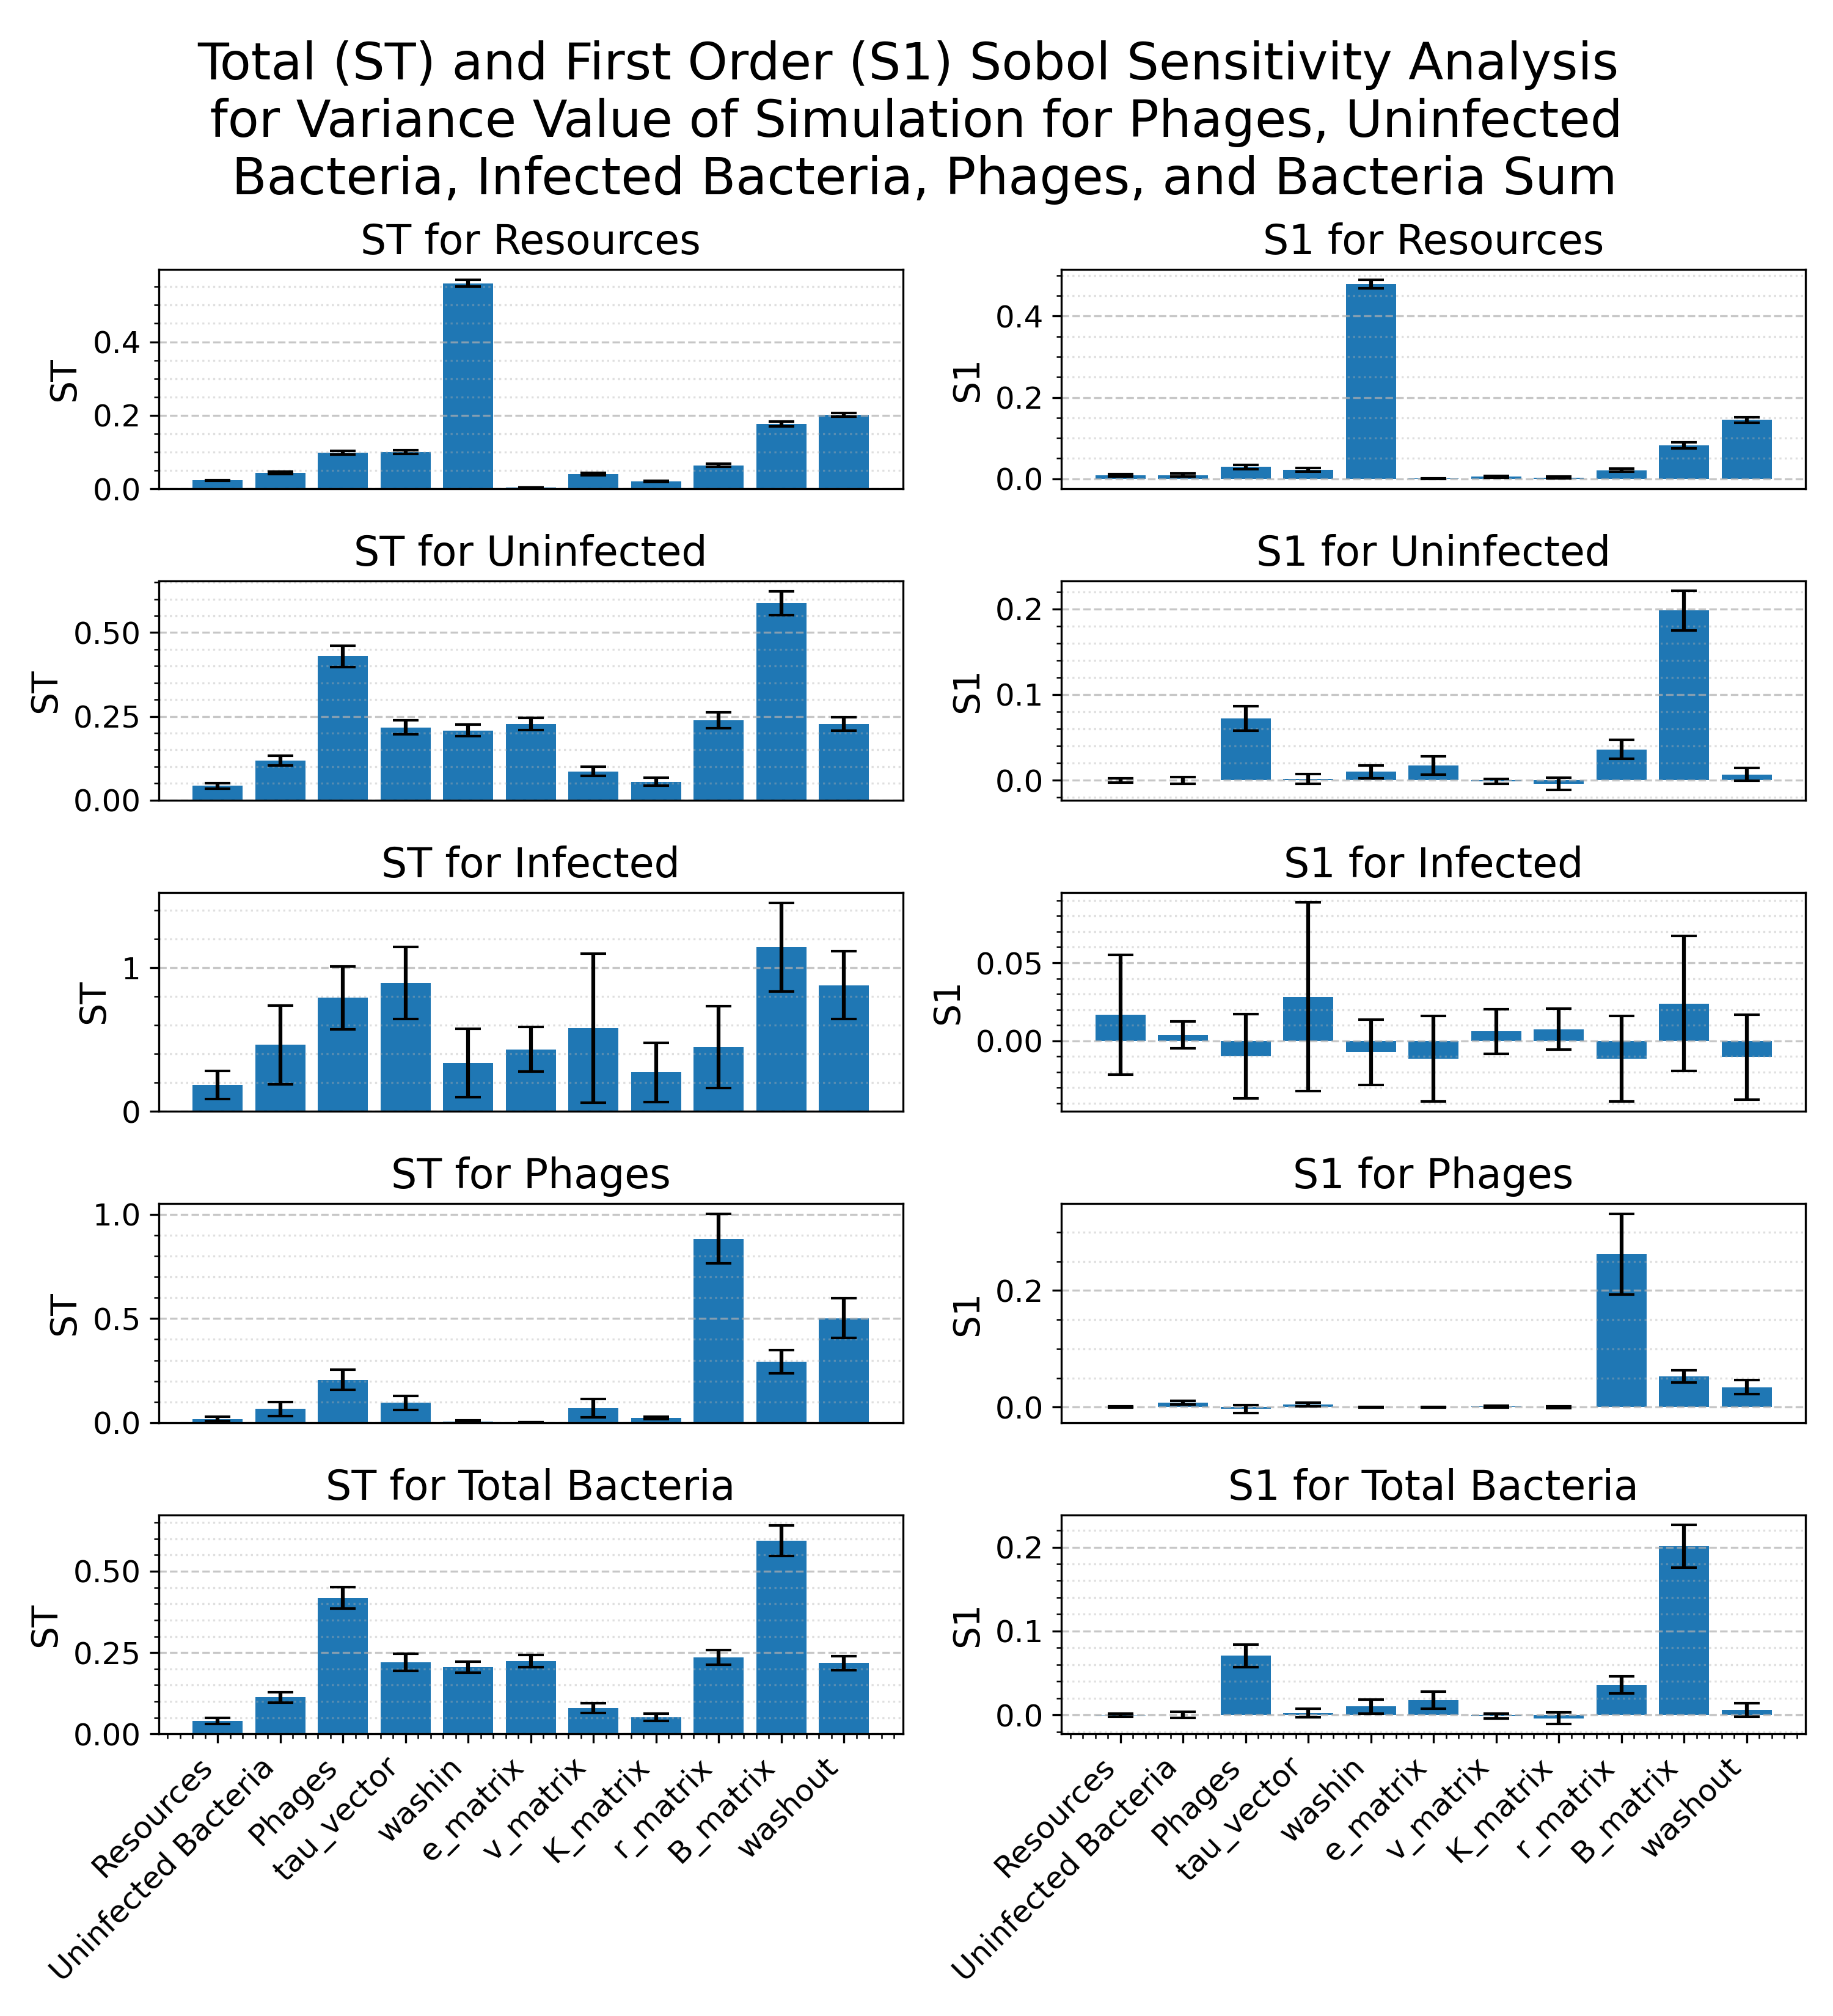
\includegraphics[width=\linewidth]{Plots/Created/SOBOL_analysis_1748084143_Variance.png}
        \caption{
            The $ST$ and $S1$ order sensitivity for the variance of Resource, Uninfected, Infected, Phage, and Total Bacteria. 
        }
        \label{fig:created:SOBOL_variance}
    \end{subfigure}
    \caption{
        The three default SOBOL analyses from the dashboard for the $1\times 1 \times 1$ golden model. 
        The data was saved from the dashboard and replotted using Matplotlib for a nicer plot and layout. 
        The results between the final, average, and variance value are nearly identical. 
        The values used for this SOBOL test can be found in \Cref{tab:appendixE:SOBOL_analysis_values}. 
        }
    \label{fig:created:SOBOL_default}
\end{figure}

\subsection{Custom SOBOL Analysis - Peak Value and Peak Time}
Due to the similarity of the final, average, and variance value, a custom SOBOL analysis that isn't included in the dashboard might result in a different SOBOL analysis result. 
As such, the peak value and the time of the peak of the population is measured. 
The peak is defined as the point where the population reaches 95\% of its absolute maximum value. 
The time of the peak is measured at the point in time that the population reaches 95\% of the maximum value. 
This removes unintended side effects of the simulation. 
For populations that are only increasing in value, this prevents the measured peak from bunching up at the end of the simulation, skewing the data. 
As the peak is defined at 95\% of the absolute maximum value, populations that have a faster increase on population count at the end will have a time value closer towards the end of the simulation. 
For populations that reach a plateau, the 95\% rule will push the peak time towards the beginning of the simulation, while still "respecting" the absolute final value since $95\% \approx 100\%$. 

\begin{figure}
    \centering
    \begin{subfigure}{0.49\linewidth}
        \centering
        \captionsetup{width=1\linewidth}
        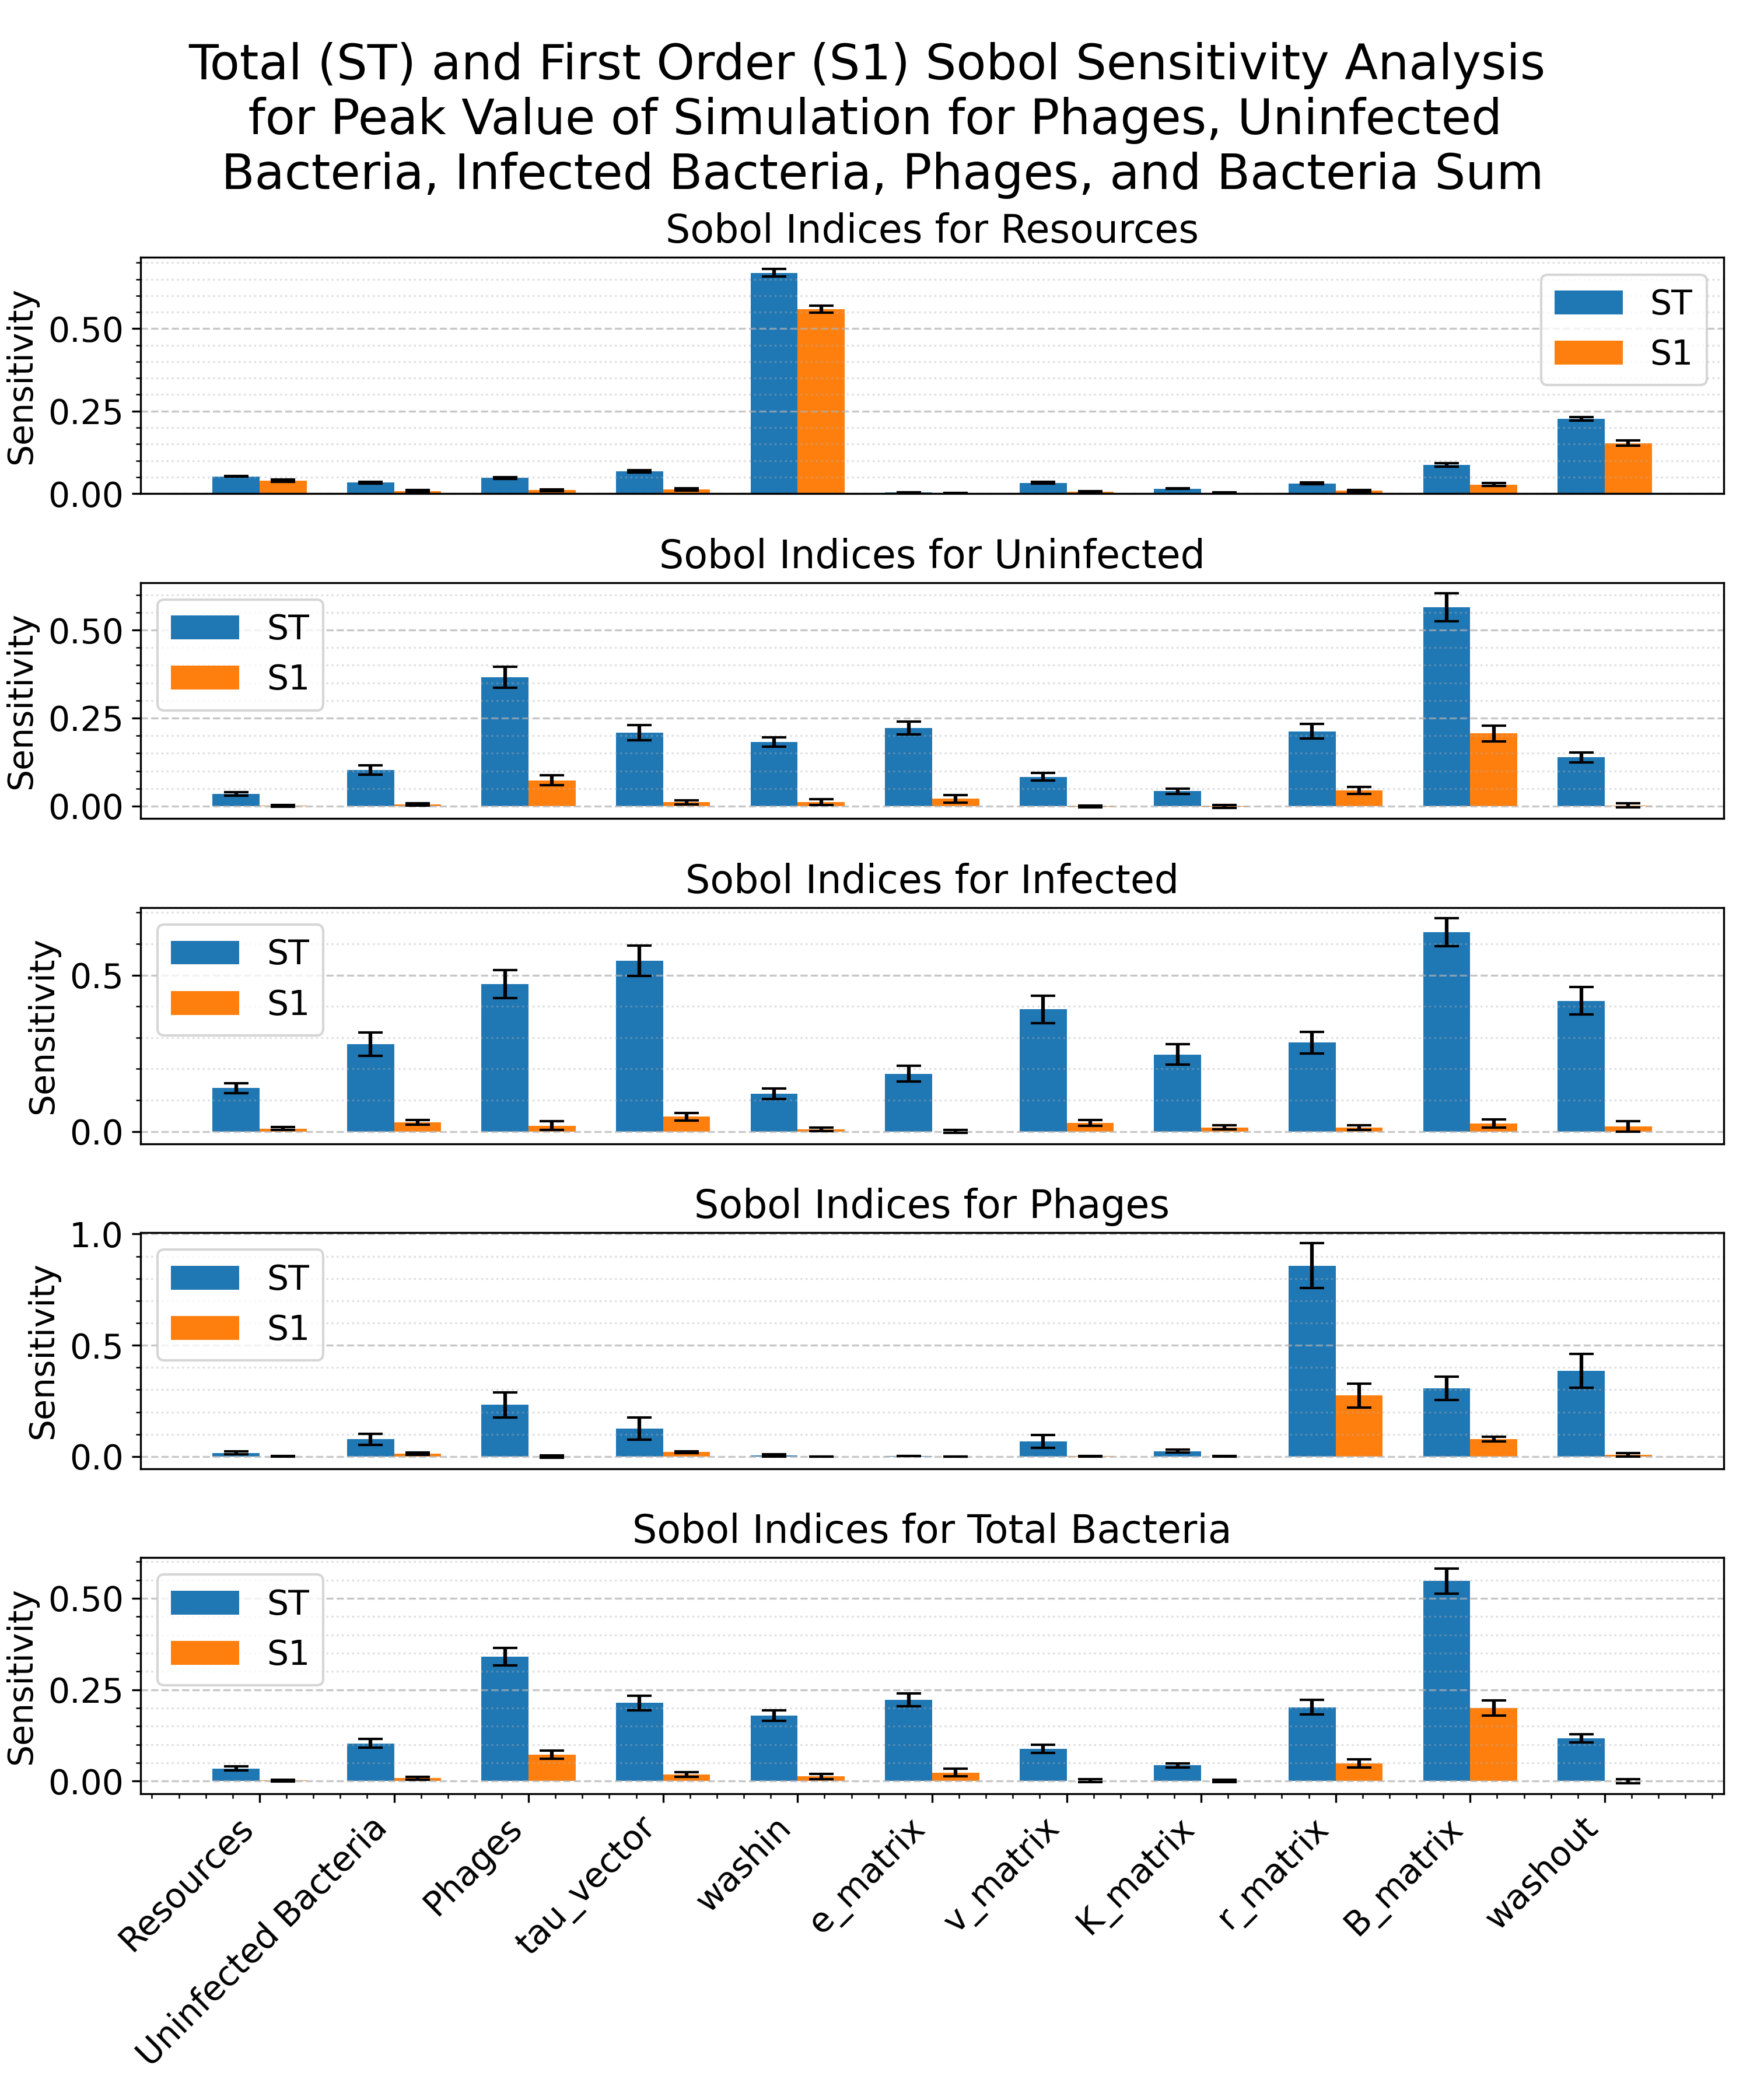
\includegraphics[width=\linewidth]{Plots/Created/SOBOL_analysis_1748084143_Peak.png}
        \caption{
            The total and first order sensitivity for the golden model for 95\% of the max value reached of the Resource, Uninfected, Infected, Phage, and Total Bacteria population count. 
        }
        \label{fig:created:SOBOL_peak}
    \end{subfigure}
    \hfill
    \begin{subfigure}{0.49\linewidth}
        \centering
        \captionsetup{width=1\linewidth}
        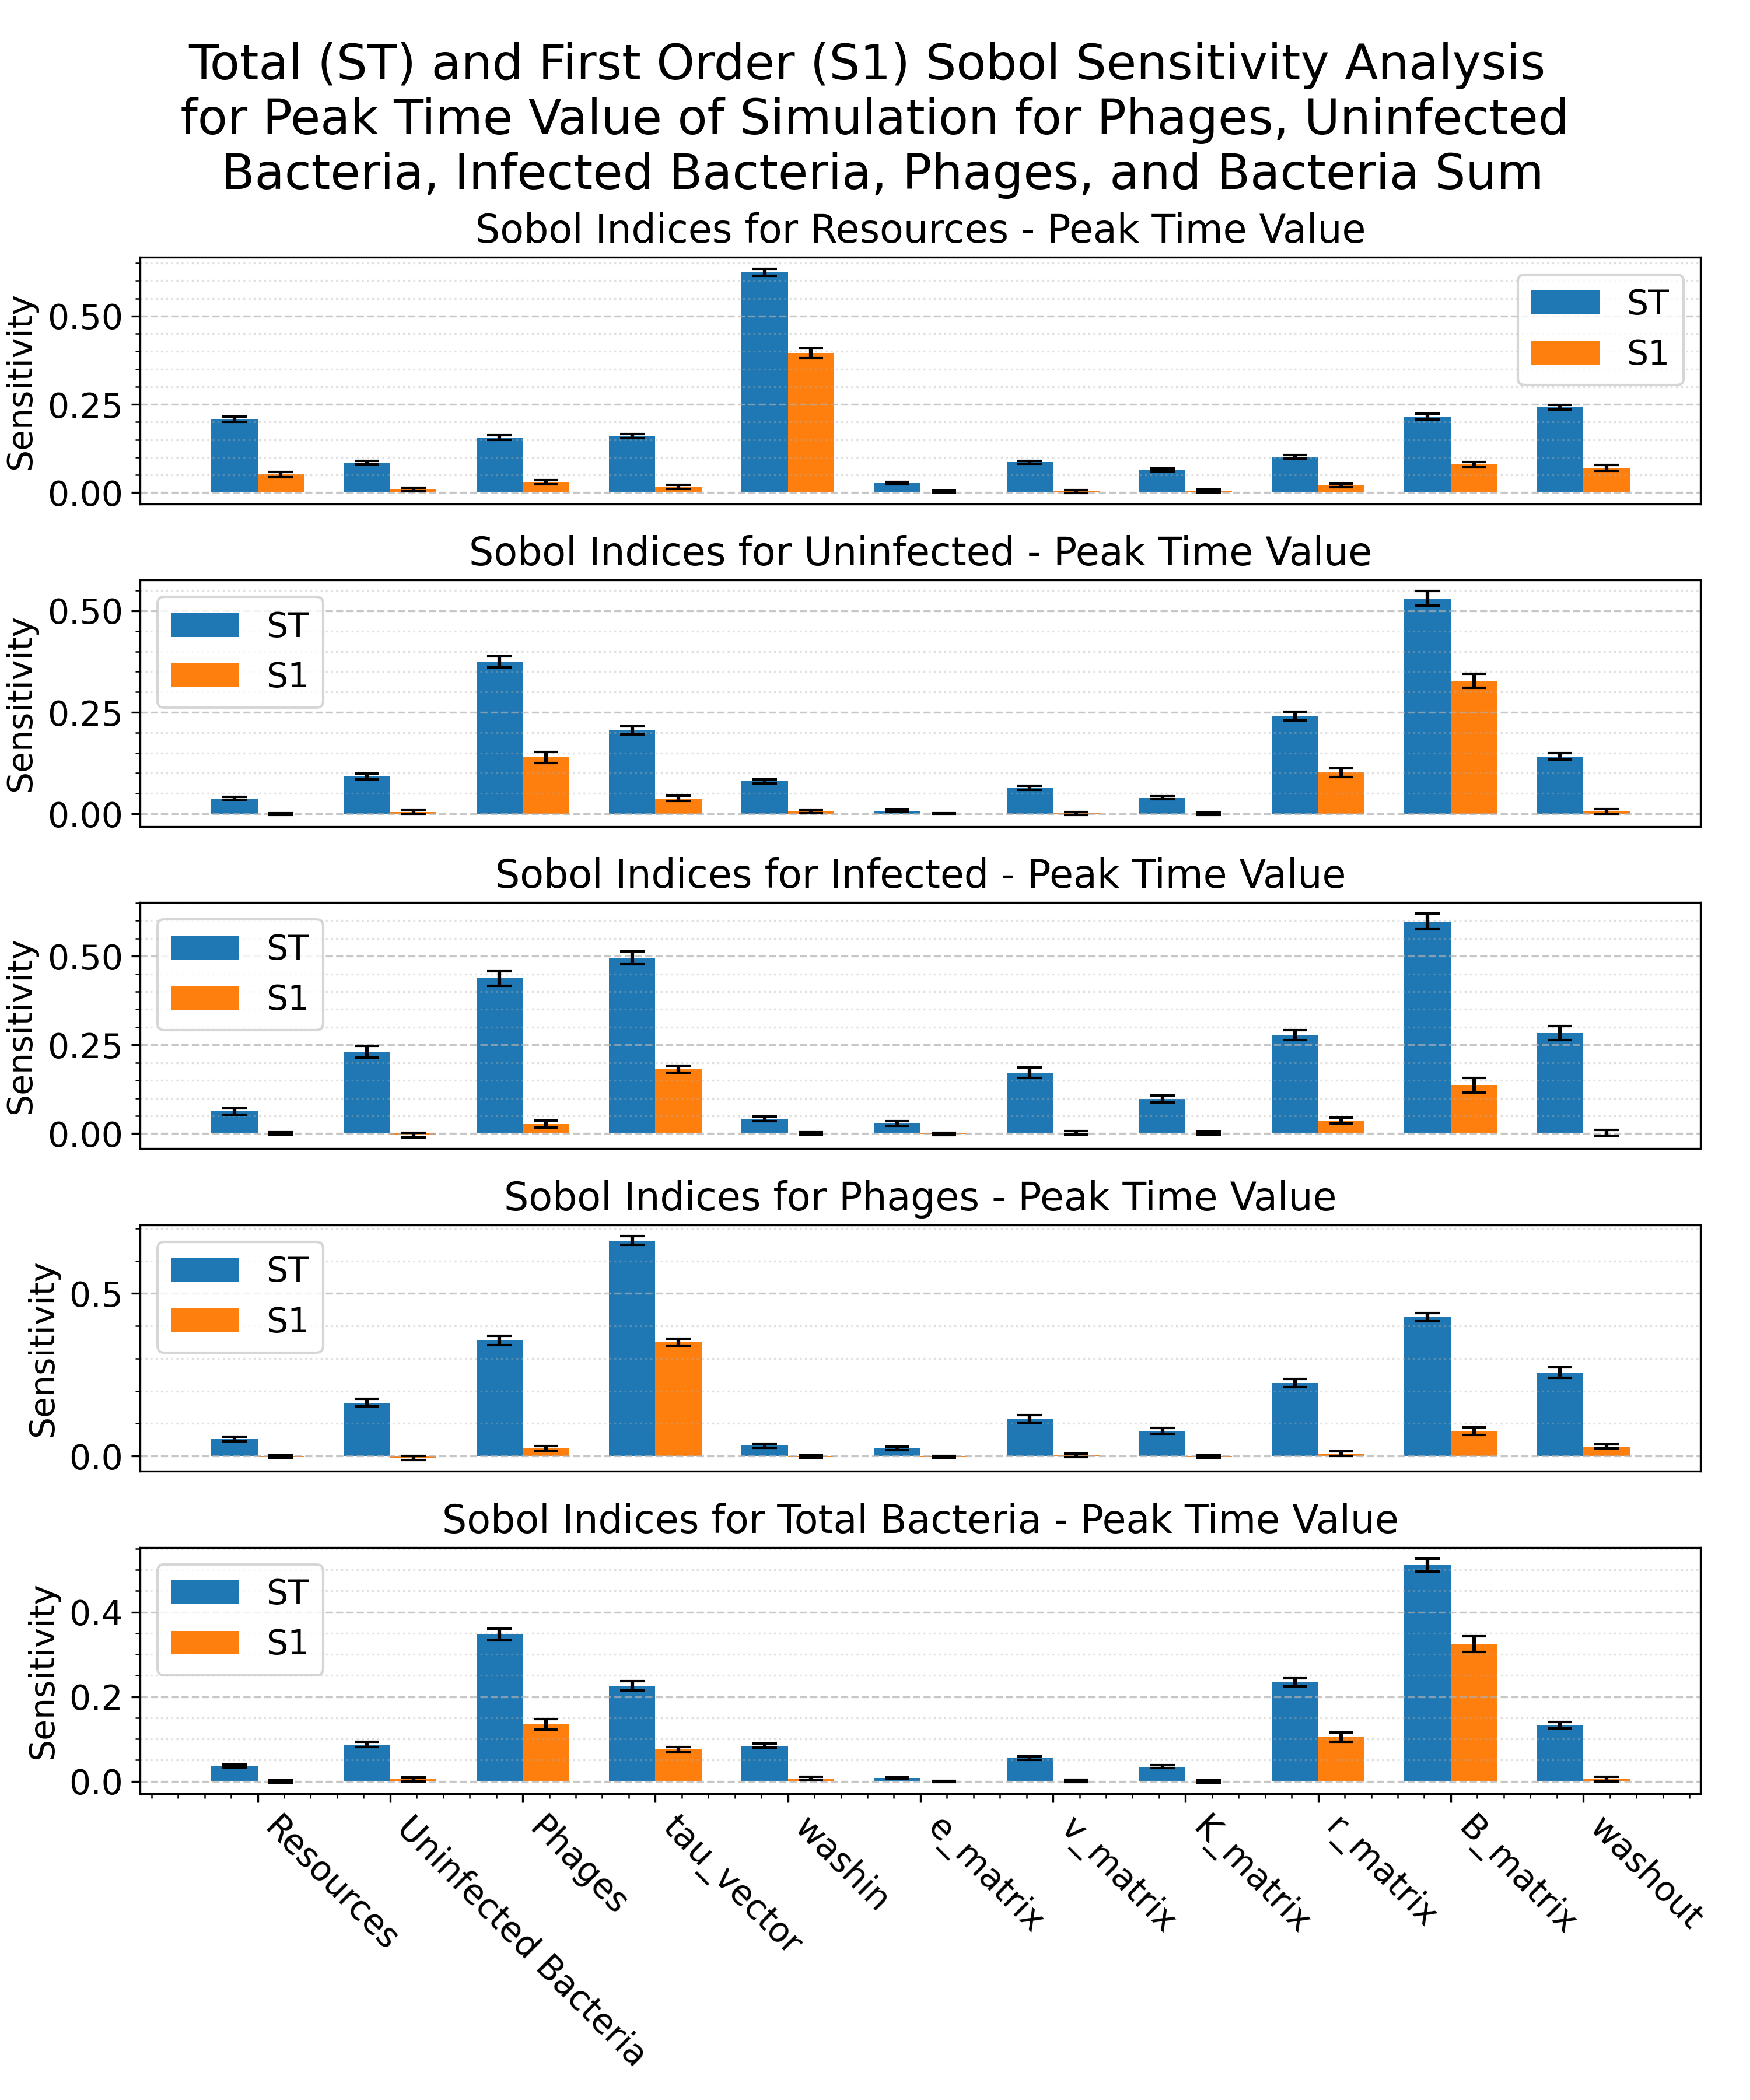
\includegraphics[width=\linewidth]{Plots/Created/SOBOL_analysis_1748084143_Peak_Time.png}
        \caption{
            The total and first order sensitivity for the golden model for the time at which 95\% of the max value occurred of the Resource, Uninfected, Infected, Phage, and Total Bacteria population value. 
        }
        \label{fig:created:SOBOL_peak_time}
        \end{subfigure}
    \caption{
        The three default SOBOL analyses from the dashboard for the $1\times 1 \times 1$ golden model. 
        The data was saved from the dashboard and replotted using Matplotlib for a nicer plot and layout. 
        The same randomly selected data used in \Cref{fig:created:SOBOL_default} was used here, and a custom analysis was run on the saved data to create these plots. 
        The values used for this SOBOL test can be found in \Cref{tab:appendixE:SOBOL_analysis_values}. 
    }
    \label{fig:created:SOBOL_custom}
\end{figure}
